\documentclass{article}

\usepackage{graphicx,epsfig,psfrag,rotate,pstool,xcolor}
\usepackage{amsmath,amsfonts,amssymb,latexsym,multicol}
\usepackage{setspace,enumerate,enumitem,ifthen,subfig}
\usepackage[portuges]{babel}

\usepackage[printwatermark]{xwatermark}
\usepackage{hyperref,framed,tcolorbox}
\usepackage{siunitx,multicol}
\usepackage{tikz}

\usepackage[utf8]{inputenc}
\usepackage[algo2e,english,onelanguage,algoruled]{algorithm2e}
\usepackage[margin=1.5cm]{geometry}
\usepackage{calrsfs}
\renewcommand{\rmdefault}{pplx}
\usepackage{eulervm}
\DeclareMathAlphabet{\mathcal}{OMS}{zplm}{m}{n}

\newcommand{\R}{\mathbb{R}}
\newcommand{\C}{\mathbb{C}}
\newcommand{\N}{\mathbb{N}}
\newcommand{\T}{\mathsf{T}}
\renewcommand{\d}{\mathrm{d}}
\newcommand{\BOX}[2]{\framebox[#1cm]{\rule{0mm}{#2cm}}}

\newwatermark[pagex={2},fontfamily=bch,color=gray!25,angle=45,scale=3,xpos=-2,ypos=-2]{RASCUNHO}


\begin{document}
%\hrule
\thispagestyle{empty}
\begin{tcolorbox}[colframe=black,colback=gray!20,arc=0pt]
\begin{center}
{\sc\Large Universidade Estadual de Campinas} \vspace{0.5cm} \\
{\sc \large Faculdade de Engenharia Elétrica e de Computação}
\end{center}
\end{tcolorbox}


%\begin{minipage}[l]{0.85\textwidth}
%{\sc \Large Universidade Estadual de Campinas} \vspace{0.5cm} \\
%{\sc \large Faculdade de Engenharia Elétrica e de Computação}
%\end{minipage}
%\begin{minipage}[c]{0.15\textwidth}
%\includegraphics[width=0.8\textwidth]{unicamp.eps}
%\end{minipage}

\noindent
\hrulefill
\fbox{\rule[-2mm]{0mm}{6mm}\sc {\bf EA044 -- Turma U -- Prova II}}
\hspace{-2.4mm}
\hrulefill
\fbox{\rule[-2mm]{0mm}{6mm} {\bf 28/11/2018}}
\hspace{-2.4mm}
\hrulefill

\vspace{1cm}

\noindent
    \framebox[14cm]{\rule{0mm}{1cm}{\bf Nome \hfill}}
	\hfill
	\framebox[3.5cm][l]{\rule{0mm}{1cm}{\bf RA}}

\vspace{1cm}

\begin{center}
    \begin{tabular}{|c||c|c|c|c|c|c|c|c|}
      \hline
                 & $\phantom{m}${\bf Q1}$\phantom{m}$ & $\phantom{m}${\bf Q2}$\phantom{m}$ & $\phantom{m}${\bf Q3}$\phantom{m}$ & $\phantom{m}${\bf Q4}$\phantom{m}$ & $\phantom{m}${\bf Q5}$\phantom{m}$ & $\phantom{m}${\bf Q6}$\phantom{m}$ & $\phantom{m}${\bf Total}$\phantom{m}$ \\
      \hline
                 &          &          &          &          &                &&                 \\
      {\bf Nota} &          &          &          &          &                  &&               \\
                 &          &          &          &          &                    &&             \\
      \hline
    \end{tabular}
\end{center}

\vspace{2cm}

%\noindent
%\hrulefill
%\fbox{\rule[-2mm]{0mm}{6mm}\sc {\bf Instruções}}
%\hspace{-2.4mm}
%\hrulefill

\noindent \hrulefill
\begin{center}
\begin{tcolorbox}[colframe=black,width =7cm,colback=gray!20,arc=0pt]
\centering {\sc {\bf Instruções}}
\end{tcolorbox}
\end{center}

\begin{multicols}{2}
\begin{itemize}
\item Esta prova tem {\bf 06 questões} distribuídas em {\bf 10 páginas}. A {\bf nota máxima} da prova é de {\bf 10,0 pontos}.
\item Cada questão deve ser resolvida, de forma {\bf organizada}, {\bf clara} e {\bf formal} no espaço indicado. Estes critérios fazem parte da avaliação.
\item Utilize a folha de almaço fornecida para rascunhos.
\item Não destaque as folhas deste caderno.
%\item Não é permitida a consulta a qualquer material.
\item É permitida a consulta a uma folha manuscrita em papel A4, que deve ser entregue juntamente com a prova.
\item Não é permitido o uso de calculadoras.
\item Qualquer tentativa de fraude, se detectada durante ou após a realização da prova, implicará em nota {\bf zero} para todos os envolvidos, além das penalidades disciplinares previstas no Regimento Geral da Unicamp (Arts. 226 -- 237).
\item A duração total da prova é de \textbf{120 minutos}.
\end{itemize}
\end{multicols}

\noindent \hrulefill

\pagebreak
\phantom{m} \thispagestyle{empty}

\pagebreak

\begin{enumerate}[label=$\blacktriangleright$ {\bf Questão \arabic*:},series=exerc,align=left]
\item {\bf (1.0pt)} Recentemente, a Internet parou para discutir a tabela de preços de um (agora famoso) restaurante em Hong Kong. Este restaurante, que serve apenas asas de frango em seu menu, pratica os preços de diversos {\em combos} conforme a figura a seguir:

\begin{figure}[h]
\centering
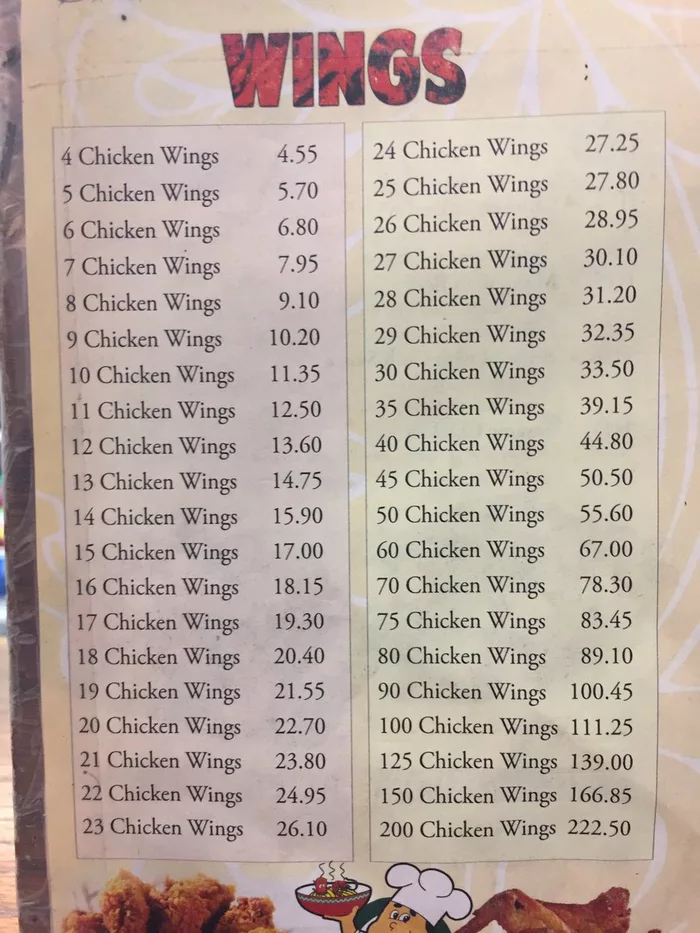
\includegraphics[width=0.4\textwidth]{wings.png}
\caption{Tabela de preços} \label{fig1}
\end{figure}

Você, um astuto estudante de otimização, desejando economizar, observa que o dono do restaurante não tem uma política de preços (HK\$/asa de frango) muito clara. Por exemplo, se você deseja comprar 60 asas de frango, é mais barato comprar dois {\em combos}, um de 50 e um de 10, em vez do {\em combo} de 60 asas. Desenvolva um problema de otimização que, dada a quantidade inteira $m$ de asas de frango desejada, faça a escolha ótima de quais {\em combos} devem ser adquiridos para que o custo total seja minimizado.

\begin{framed}
{\bf Resolução:}
Sejam $x_i$ o número de combos da posição $i$, $n_i$ o número de asas de frango que o $i$-ésimo combo contém e $c_i$ o custo do $i$-ésimo combo, então podemos formular o problema como
\[
\begin{array}{rl}
  \min & \sum_i c_i x_i \\
  \text{sujeito a} & \sum_i n_i x_i \ge m,\\
  & x_i \in \mathbb{N} \quad \forall i.
\end{array}
\]
\vspace{4cm}
\end{framed}

\pagebreak

\item Considere o seguinte problema da mochila
\[
\begin{array}{rl}
  \max & 50x_1 + 60x_2 + 140 x_3 + 40x_4 \\
  \text{sujeito a} & 5x_1 + 10 x_2 + 20 x_3 + 20 x_4 \leq 30,\\
  & x_1,x_2,x_3,x_4 \in \mathbb{B} \triangleq \{0,1\}.
\end{array}
\]
\begin{enumerate}[label=(\alph*),series=q2]
\item {\bf (1.0pt)} Formule a relaxação deste problema removendo-se a restrição de integralidade, ou seja, o {\em problema da mochila fracionário} associado a este. Mostre como obter a solução ótima deste problema e determine esta solução. Dica: a estratégia gulosa clássica funciona para o problema da mochila fracionário.
\begin{framed}
{\bf Resolução:}
\[
\begin{array}{rl}
  \max & 50x_1 + 60x_2 + 140 x_3 + 40x_4 \\
  \text{sujeito a} & 5x_1 + 10 x_2 + 20 x_3 + 20 x_4 \leq 30,\\
  & x_1,x_2,x_3,x_4 \in [0,1].
\end{array}
\]
A utilidade por peso dos itens é dada por $50/5 = 10$, $60/10 = 6$, $140/20 = 7$ e $40/20 = 2$ para o primeiro, segundo, terceiro e quarto item, respectivamente. Logo, devemos colocar o máximo possível dos itens na ordem 1, 3, 2, 4 até atingir o peso máximo. Dessa forma, obtemos a solução $x^\star = [1, 1/2, 1, 0]^\T$.
\end{framed}

\item {\bf (1.5pt)} Resolva o problema acima usando {\em branch \& bound}. Construa a árvore de B\&B e explique quais nós fornecem candidatas a solução ótima e quais nós podem ser eliminados por estas candidatas. Resolva cada subproblema usando a estratégia gulosa usada acima.
\begin{framed}
{\bf Resolução:}
\begin{center}
    

\tikzset{every picture/.style={line width=0.75pt}} %set default line width to 0.75pt        

\begin{tikzpicture}[x=0.75pt,y=0.75pt,yscale=-1,xscale=1]
%uncomment if require: \path (0,482.45454597473145); %set diagram left start at 0, and has height of 482.45454597473145

%Straight Lines [id:da8893535372195869] 
\draw    (324.9,127.52) -- (183.9,177.52) ;


%Straight Lines [id:da06977988794497159] 
\draw    (324.9,127.52) -- (455.9,177.52) ;


%Straight Lines [id:da5441471698763001] 
\draw    (417.9,302.52) -- (277.9,351.52) ;


%Straight Lines [id:da5406490821861696] 
\draw    (416.9,302.52) -- (546.9,350.52) ;



% Text Node
\draw    (322, 21) circle [x radius= 17.8, y radius= 17.8]   ;
\draw (322,21) node [scale=1]  {$P_{0}$};
% Text Node
\draw    (206.5,38.5) -- (437.5,38.5) -- (437.5,127.5) -- (206.5,127.5) -- cycle  ;
\draw (322,83) node   {$\quad x^{( 0)} =\begin{bmatrix}
1\\
1/2\\
1\\
0
\end{bmatrix} ,\ f^{\text{T}} x^{( 0)} =220\quad $};
% Text Node
\draw    (185, 196) circle [x radius= 17.8, y radius= 17.8]   ;
\draw (185,196) node   {$P_{1}$};
% Text Node
\draw  [fill={rgb, 255:red, 208; green, 2; blue, 27 }  ,fill opacity=0.6 ]  (70.5,214.5) -- (301.5,214.5) -- (301.5,303.5) -- (70.5,303.5) -- cycle  ;
\draw (186,259) node   {$\quad x^{( 1)} =\begin{bmatrix}
1\\
0\\
1\\
1/4
\end{bmatrix} ,\ f^{\text{T}} x^{( 1)} =200\quad $};
% Text Node
\draw    (457, 195) circle [x radius= 17.8, y radius= 17.8]   ;
\draw (457,195) node   {$P_{2}$};
% Text Node
\draw    (341.5,213.5) -- (572.5,213.5) -- (572.5,302.5) -- (341.5,302.5) -- cycle  ;
\draw (457,258) node   {$\quad x^{( 2)} =\begin{bmatrix}
1\\
1\\
3/4\\
0
\end{bmatrix} ,\ f^{\text{T}} x^{( 2)} =215\quad $};
% Text Node
\draw (442,153) node   {$x_{2} \geq 1$};
% Text Node
\draw (215,151) node   {$x_{2} \leq 0$};
% Text Node
\draw    (278, 371) circle [x radius= 19.45, y radius= 19.45]   ;
\draw (278,371) node   {$P_{21}$};
% Text Node
\draw  [fill={rgb, 255:red, 208; green, 2; blue, 27 }  ,fill opacity=0.6 ]  (157.5,390.5) -- (400.5,390.5) -- (400.5,479.5) -- (157.5,479.5) -- cycle  ;
\draw (279,435) node   {$\quad x^{( 21)} =\begin{bmatrix}
1\\
1\\
0\\
3/4
\end{bmatrix} ,\ f^{\text{T}} x^{( 21)} =140\quad $};
% Text Node
\draw    (547, 370) circle [x radius= 19.45, y radius= 19.45]   ;
\draw (547,370) node   {$P_{22}$};
% Text Node
\draw  [fill={rgb, 255:red, 126; green, 211; blue, 33 }  ,fill opacity=0.8 ]  (435,389.5) -- (659,389.5) -- (659,478.5) -- (435,478.5) -- cycle  ;
\draw (547,434) node   {$\quad x^{( 22)} =\begin{bmatrix}
0\\
1\\
1\\
0
\end{bmatrix} ,\ f^{\text{T}} x^{( 22)} =200\quad $};
% Text Node
\draw (470,341) node   {$x_{3} \geq 1$};
% Text Node
\draw (361,341) node   {$x_{3} \leq 0$};


\end{tikzpicture}

\end{center}
Obtemos solução inteira com o nó $P_{22}$. Como os nós $P_1$ e $P_{21}$ fornecem valores ótimos iguais ou piores, podemos eliminá-los. 
\end{framed}
% \pagebreak
% \begin{framed}
% {\bf Resolução:}
% \vspace{23cm}
% \end{framed}

\end{enumerate}
\end{enumerate}

\pagebreak

\begin{enumerate}[resume*=exerc]
\item {\bf (1.5pt)} Após uma (complicada) festa universitária, muitos estudantes tiveram que ir para a emergência de um hospital. No total, 150 alunos têm que receber, via transfusão, uma bolsa de sangue cada. O hospital tem 155 bolsas disponíveis. A tabela a seguir ilustra a distribuição de tipo sanguíneo dos estudantes e das bolsas disponíveis.

    \begin{center}
      \begin{tabular}{|l||c|c|c|c|}
        \hline
        % after \\: \hline or \cline{col1-col2} \cline{col3-col4} ...
        Tipo & A & B & O & AB \\
        \hline\hline
        Bolsas & 44 & 31 & 42 & 38 \\
        \hline
        Alunos & 41 & 36 & 30 & 43 \\
        \hline
      \end{tabular}
    \end{center}

    Lembre que pacientes do tipo A podem receber sangue de tipo A ou tipo O; pacientes do tipo B podem receber apenas sangue de tipo B ou O; pacientes do tipo O apenas recebem sangue de tipo O; pacientes de tipo AB podem receber qualquer um dos tipos de sangue.

    Você, como gerente do hospital, deve analisar se o estoque do hospital é suficiente para atender a esta demanda; além disso, seu objetivo é atender a todos os alunos usando o menor número possível de bolsas de sangue do doador universal (tipo O). Modele este problema como um problema de transporte {\bf balanceado} (ou seja, esboce a rede de fluxo das fontes -- bolsas -- para os destinos -- alunos); formule, também, o PLI que deve ser resolvido neste caso. Você não precisa resolver o problema.
\begin{framed}
{\bf Resolução:}
Note que o número de bolsas de sangue supera em 5 o número de alunos, logo é necessário criar um nó com demanda 5 para o problema ficar balanceado. Esse novo nó representa o número de bolsas que não serão utilizadas. Todas as arestas tem peso 0, exceto a aresta $O\rightarrow R$.

\begin{center}
    

\tikzset{every picture/.style={line width=0.75pt}} %set default line width to 0.75pt        

\begin{tikzpicture}[x=0.75pt,y=0.75pt,yscale=-1,xscale=1]
%uncomment if require: \path (0,375.6363525390625); %set diagram left start at 0, and has height of 375.6363525390625

%Shape: Circle [id:dp7783632791548247] 
\draw   (61,45) .. controls (61,31.19) and (72.19,20) .. (86,20) .. controls (99.81,20) and (111,31.19) .. (111,45) .. controls (111,58.81) and (99.81,70) .. (86,70) .. controls (72.19,70) and (61,58.81) .. (61,45) -- cycle ;
%Shape: Circle [id:dp3825720642161514] 
\draw   (60.33,106) .. controls (60.33,92.19) and (71.53,81) .. (85.33,81) .. controls (99.14,81) and (110.33,92.19) .. (110.33,106) .. controls (110.33,119.81) and (99.14,131) .. (85.33,131) .. controls (71.53,131) and (60.33,119.81) .. (60.33,106) -- cycle ;
%Shape: Circle [id:dp8770196169464097] 
\draw   (61,165) .. controls (61,151.19) and (72.19,140) .. (86,140) .. controls (99.81,140) and (111,151.19) .. (111,165) .. controls (111,178.81) and (99.81,190) .. (86,190) .. controls (72.19,190) and (61,178.81) .. (61,165) -- cycle ;
%Shape: Circle [id:dp7061290690327051] 
\draw   (61,226) .. controls (61,212.19) and (72.19,201) .. (86,201) .. controls (99.81,201) and (111,212.19) .. (111,226) .. controls (111,239.81) and (99.81,251) .. (86,251) .. controls (72.19,251) and (61,239.81) .. (61,226) -- cycle ;
%Shape: Circle [id:dp45906670482832146] 
\draw   (240,45) .. controls (240,31.19) and (251.19,20) .. (265,20) .. controls (278.81,20) and (290,31.19) .. (290,45) .. controls (290,58.81) and (278.81,70) .. (265,70) .. controls (251.19,70) and (240,58.81) .. (240,45) -- cycle ;
%Shape: Circle [id:dp8837516273367831] 
\draw   (239.33,106) .. controls (239.33,92.19) and (250.53,81) .. (264.33,81) .. controls (278.14,81) and (289.33,92.19) .. (289.33,106) .. controls (289.33,119.81) and (278.14,131) .. (264.33,131) .. controls (250.53,131) and (239.33,119.81) .. (239.33,106) -- cycle ;
%Shape: Circle [id:dp538822308803613] 
\draw   (240,165) .. controls (240,151.19) and (251.19,140) .. (265,140) .. controls (278.81,140) and (290,151.19) .. (290,165) .. controls (290,178.81) and (278.81,190) .. (265,190) .. controls (251.19,190) and (240,178.81) .. (240,165) -- cycle ;
%Shape: Circle [id:dp020672157708870653] 
\draw   (240,226) .. controls (240,212.19) and (251.19,201) .. (265,201) .. controls (278.81,201) and (290,212.19) .. (290,226) .. controls (290,239.81) and (278.81,251) .. (265,251) .. controls (251.19,251) and (240,239.81) .. (240,226) -- cycle ;
%Shape: Circle [id:dp4084620712660494] 
\draw   (240,286) .. controls (240,272.19) and (251.19,261) .. (265,261) .. controls (278.81,261) and (290,272.19) .. (290,286) .. controls (290,299.81) and (278.81,311) .. (265,311) .. controls (251.19,311) and (240,299.81) .. (240,286) -- cycle ;
%Straight Lines [id:da8111545967921532] 
\draw    (111,45) -- (238,45) ;
\draw [shift={(240,45)}, rotate = 180] [color={rgb, 255:red, 0; green, 0; blue, 0 }  ][line width=0.75]    (10.93,-3.29) .. controls (6.95,-1.4) and (3.31,-0.3) .. (0,0) .. controls (3.31,0.3) and (6.95,1.4) .. (10.93,3.29)   ;

%Straight Lines [id:da8327232458392688] 
\draw    (110.33,106) -- (237.33,106) ;
\draw [shift={(239.33,106)}, rotate = 180] [color={rgb, 255:red, 0; green, 0; blue, 0 }  ][line width=0.75]    (10.93,-3.29) .. controls (6.95,-1.4) and (3.31,-0.3) .. (0,0) .. controls (3.31,0.3) and (6.95,1.4) .. (10.93,3.29)   ;

%Straight Lines [id:da6154179128106005] 
\draw    (111,165) -- (238,165) ;
\draw [shift={(240,165)}, rotate = 180] [color={rgb, 255:red, 0; green, 0; blue, 0 }  ][line width=0.75]    (10.93,-3.29) .. controls (6.95,-1.4) and (3.31,-0.3) .. (0,0) .. controls (3.31,0.3) and (6.95,1.4) .. (10.93,3.29)   ;

%Straight Lines [id:da8839462157709732] 
\draw    (111,226) -- (238,226) ;
\draw [shift={(240,226)}, rotate = 180] [color={rgb, 255:red, 0; green, 0; blue, 0 }  ][line width=0.75]    (10.93,-3.29) .. controls (6.95,-1.4) and (3.31,-0.3) .. (0,0) .. controls (3.31,0.3) and (6.95,1.4) .. (10.93,3.29)   ;

%Straight Lines [id:da8434825745308232] 
\draw    (111.33,165.5) -- (238.52,224.66) ;
\draw [shift={(240.33,225.5)}, rotate = 204.94] [color={rgb, 255:red, 0; green, 0; blue, 0 }  ][line width=0.75]    (10.93,-3.29) .. controls (6.95,-1.4) and (3.31,-0.3) .. (0,0) .. controls (3.31,0.3) and (6.95,1.4) .. (10.93,3.29)   ;

%Straight Lines [id:da8495205722118699] 
\draw    (110.33,106) -- (238.53,224.64) ;
\draw [shift={(240,226)}, rotate = 222.78] [color={rgb, 255:red, 0; green, 0; blue, 0 }  ][line width=0.75]    (10.93,-3.29) .. controls (6.95,-1.4) and (3.31,-0.3) .. (0,0) .. controls (3.31,0.3) and (6.95,1.4) .. (10.93,3.29)   ;

%Straight Lines [id:da06435270243336921] 
\draw    (111,45) -- (238.84,224.37) ;
\draw [shift={(240,226)}, rotate = 234.52] [color={rgb, 255:red, 0; green, 0; blue, 0 }  ][line width=0.75]    (10.93,-3.29) .. controls (6.95,-1.4) and (3.31,-0.3) .. (0,0) .. controls (3.31,0.3) and (6.95,1.4) .. (10.93,3.29)   ;

%Straight Lines [id:da17003413818026725] 
\draw    (111.33,165.5) -- (237.85,106.35) ;
\draw [shift={(239.67,105.5)}, rotate = 514.94] [color={rgb, 255:red, 0; green, 0; blue, 0 }  ][line width=0.75]    (10.93,-3.29) .. controls (6.95,-1.4) and (3.31,-0.3) .. (0,0) .. controls (3.31,0.3) and (6.95,1.4) .. (10.93,3.29)   ;

%Straight Lines [id:da06404033638226436] 
\draw    (111.67,165) -- (238.54,46.37) ;
\draw [shift={(240,45)}, rotate = 496.92] [color={rgb, 255:red, 0; green, 0; blue, 0 }  ][line width=0.75]    (10.93,-3.29) .. controls (6.95,-1.4) and (3.31,-0.3) .. (0,0) .. controls (3.31,0.3) and (6.95,1.4) .. (10.93,3.29)   ;

%Straight Lines [id:da901246443914296] 
\draw    (111,226) -- (238.19,285.16) ;
\draw [shift={(240,286)}, rotate = 204.94] [color={rgb, 255:red, 0; green, 0; blue, 0 }  ][line width=0.75]    (10.93,-3.29) .. controls (6.95,-1.4) and (3.31,-0.3) .. (0,0) .. controls (3.31,0.3) and (6.95,1.4) .. (10.93,3.29)   ;

%Straight Lines [id:da7345540978718543] 
\draw    (111,165) -- (238.54,284.63) ;
\draw [shift={(240,286)}, rotate = 223.17000000000002] [color={rgb, 255:red, 0; green, 0; blue, 0 }  ][line width=0.75]    (10.93,-3.29) .. controls (6.95,-1.4) and (3.31,-0.3) .. (0,0) .. controls (3.31,0.3) and (6.95,1.4) .. (10.93,3.29)   ;

%Straight Lines [id:da5472484314244583] 
\draw    (110.33,106) -- (238.83,284.38) ;
\draw [shift={(240,286)}, rotate = 234.23] [color={rgb, 255:red, 0; green, 0; blue, 0 }  ][line width=0.75]    (10.93,-3.29) .. controls (6.95,-1.4) and (3.31,-0.3) .. (0,0) .. controls (3.31,0.3) and (6.95,1.4) .. (10.93,3.29)   ;

%Straight Lines [id:da8997222690304656] 
\draw    (111,45) -- (239.06,284.24) ;
\draw [shift={(240,286)}, rotate = 241.84] [color={rgb, 255:red, 0; green, 0; blue, 0 }  ][line width=0.75]    (10.93,-3.29) .. controls (6.95,-1.4) and (3.31,-0.3) .. (0,0) .. controls (3.31,0.3) and (6.95,1.4) .. (10.93,3.29)   ;

%Right Arrow [id:dp21063774080903297] 
\draw   (39.05,40.65) -- (52.22,40.65) -- (52.22,35.32) -- (61,45.98) -- (52.22,56.64) -- (52.22,51.31) -- (39.05,51.31) -- cycle ;
%Right Arrow [id:dp831270604164924] 
\draw   (38.38,100.67) -- (51.55,100.67) -- (51.55,95.34) -- (60.33,106) -- (51.55,116.66) -- (51.55,111.33) -- (38.38,111.33) -- cycle ;
%Right Arrow [id:dp6978484892697405] 
\draw   (290,39.67) -- (303.17,39.67) -- (303.17,34.34) -- (311.95,45) -- (303.17,55.66) -- (303.17,50.33) -- (290,50.33) -- cycle ;
%Right Arrow [id:dp4423721304027586] 
\draw   (289.33,100.67) -- (302.51,100.67) -- (302.51,95.34) -- (311.29,106) -- (302.51,116.66) -- (302.51,111.33) -- (289.33,111.33) -- cycle ;
%Right Arrow [id:dp46301569748671456] 
\draw   (290,159.67) -- (303.17,159.67) -- (303.17,154.34) -- (311.95,165) -- (303.17,175.66) -- (303.17,170.33) -- (290,170.33) -- cycle ;
%Right Arrow [id:dp4604714725426764] 
\draw   (290,220.67) -- (303.17,220.67) -- (303.17,215.34) -- (311.95,226) -- (303.17,236.66) -- (303.17,231.33) -- (290,231.33) -- cycle ;
%Right Arrow [id:dp1774700914380689] 
\draw   (290,280.67) -- (303.17,280.67) -- (303.17,275.34) -- (311.95,286) -- (303.17,296.66) -- (303.17,291.33) -- (290,291.33) -- cycle ;
%Right Arrow [id:dp8406255494793606] 
\draw   (39.05,159.67) -- (52.22,159.67) -- (52.22,154.34) -- (61,165) -- (52.22,175.66) -- (52.22,170.33) -- (39.05,170.33) -- cycle ;
%Right Arrow [id:dp5175966416311699] 
\draw   (39.05,220.67) -- (52.22,220.67) -- (52.22,215.34) -- (61,226) -- (52.22,236.66) -- (52.22,231.33) -- (39.05,231.33) -- cycle ;

% Text Node
\draw (85,44) node   {$A$};
% Text Node
\draw (85,164) node   {$O$};
% Text Node
\draw (86,106) node   {$B$};
% Text Node
\draw (86,225) node   {$AB$};
% Text Node
\draw (264,44) node   {$A$};
% Text Node
\draw (264,164) node   {$O$};
% Text Node
\draw (265,106) node   {$B$};
% Text Node
\draw (265,225) node   {$AB$};
% Text Node
\draw (265,285) node   {$R$};
% Text Node
\draw (22,45) node   {$44$};
% Text Node
\draw (22,105) node   {$31$};
% Text Node
\draw (21.5,164) node   {$42$};
% Text Node
\draw (22,225) node   {$38$};
% Text Node
\draw (329,44) node   {$41$};
% Text Node
\draw (330,105) node   {$36$};
% Text Node
\draw (329,164) node   {$30$};
% Text Node
\draw (329,225) node   {$43$};
% Text Node
\draw (333,285) node   {$5$};
% Text Node
\draw (134,195) node [scale=0.8]  {$1$};


\end{tikzpicture}

\end{center}
Sejam $x_{i,j}$ o número de bolsas transferidas de $i\in\{A,B,O,AB\}$ para $j\in\{A,B,O,AB,R\}$, então o PLI é
\[
\begin{array}{rl}
  \max & x_{O,R} \\
  \text{sujeito a} & x_{A,A} + x_{A,AB} + x_{A,R} = 44,\\
  & x_{B,B} + x_{B,AB} + x_{B,R} = 31,\\
  & x_{O,A} + x_{O,B} + x_{O,O} + x_{O,AB} + x_{O,R} = 42,\\
  & x_{AB,AB} + x_{AB,R} = 38,\\
  & x_{A,A} + x_{O,A} = 41,\\
  & x_{B,B} + x_{O,B} = 36,\\
  & x_{O,O} = 30,\\
  & x_{A,AB} + x_{B,AB} + x_{O,AB} + x_{AB,AB} = 43,\\
  & x_{A,R} + x_{B,R} + x_{O,R} + x_{AB,R} = 5,\\
  & x_{i,j} \in \N, \quad i,j\in\{A,B,O,AB\}\times\{A,B,O,AB,R\}.
\end{array}
\]

\end{framed}


\end{enumerate}

\pagebreak

\begin{enumerate}[resume*=exerc]
\item Considere um grafo $G = (V,E)$ com $n+1$ nós $V = \{v_0,\cdots,v_n\}$ tal que, para qualquer $i \in \{1,\cdots,n\}$, existe uma aresta com peso (custo) $n$ de $v_0$ a $v_i$ e que, para qualquer $i \in \{1,\cdots,n\}$, existe uma aresta com peso $i$ entre $v_i$ e $v_{i+1}$. Um grafo desta forma está mostrado na figura abaixo.

\begin{figure}[h]
\centering
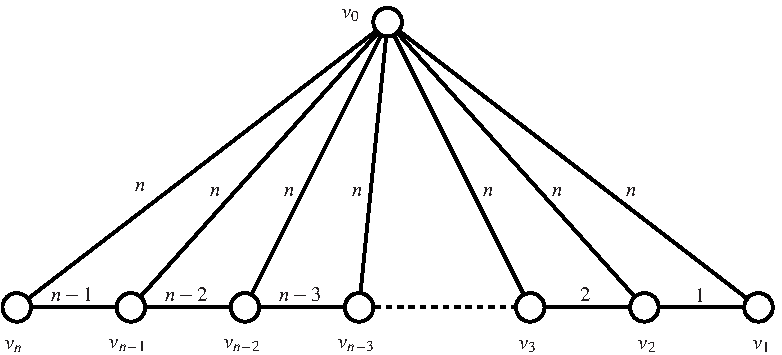
\includegraphics[width=0.6\textwidth]{agm_p2}
\caption{Grafo para a Questão 4.} \label{fig1}
\end{figure}

\begin{enumerate}[label=(\alph*),series=q4]
\item {\bf (1.0pt)} Use o algoritmo de Kruskal para determinar uma árvore geradora mínima para este grafo.
\begin{framed}
{\bf Resolução:}
\begin{center}
    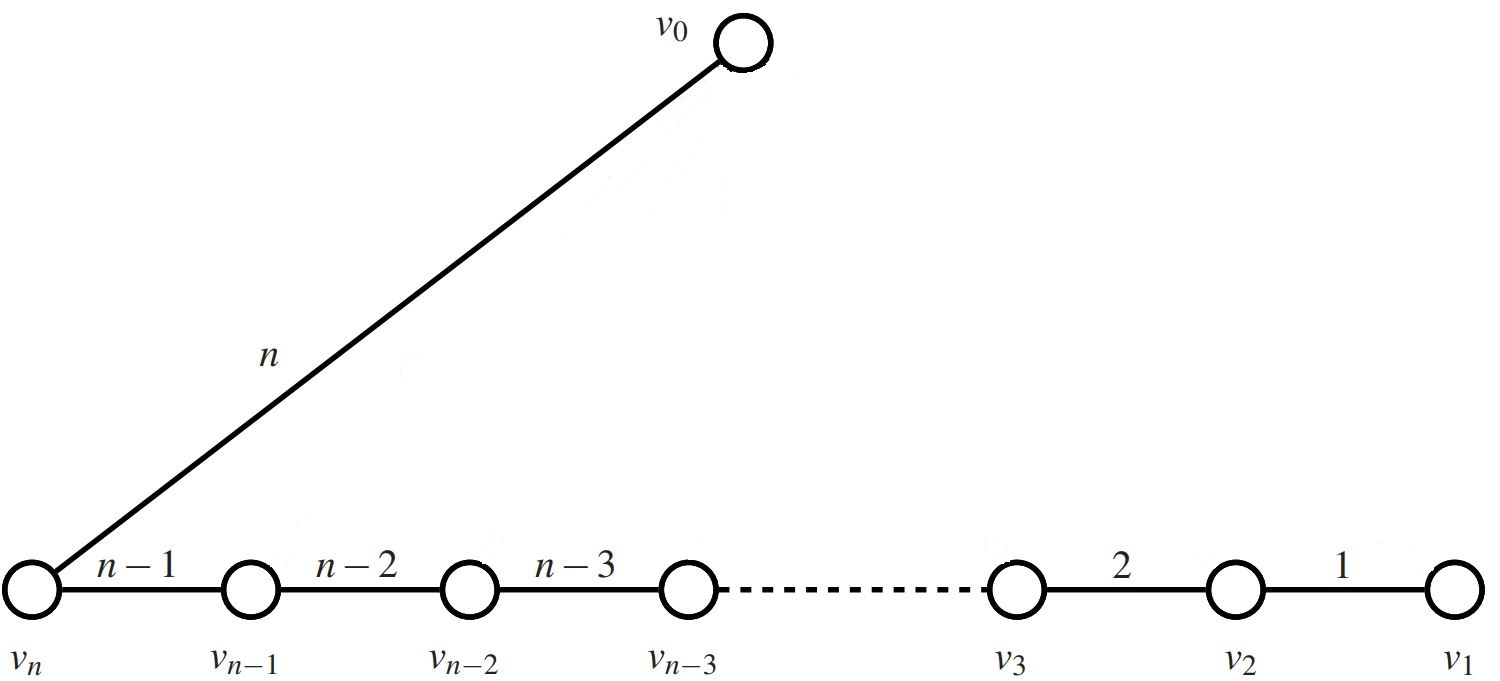
\includegraphics[width=0.6\textwidth]{4a.JPG}
\end{center}
\vspace{1cm}
\end{framed}

\item {\bf (0.5pt)} Forneça $n$ diferentes árvores geradoras mínimas para este grafo. Dica: pense nas escolhas que você tinha no item anterior.
\begin{framed}
{\bf Resolução:}
A aresta $\nu_0\leftrightarrow \nu_n$ pode ser trocada pela aresta $\nu_0\leftrightarrow \nu_i$ para todo $i\in\{1,2,\dots,n-1\}$ e a árvore continua sendo geradora mínima.
\vspace{5cm}
\end{framed}
\pagebreak
\item {\bf (1.0pt)} Considere a árvore geradora mínima que contém a aresta $(v_0,v_1)$. Para que valores de $n$ esta árvore é uma árvore de caminho mínimo a partir de $v_1$?
\begin{framed}
{\bf Resolução:}
A árvore geradora mínima coincide com a de caminho mínimo enquanto for vantajoso percorrer o caminho $\nu_1 \rightarrow \nu_2 \rightarrow \cdots \rightarrow \nu_{n-1} \rightarrow \nu_n$ ao invés de $\nu_1 \rightarrow \nu_0 \rightarrow \nu_n$, ou seja, enquanto a seguinte inequação for satisfeita
\[
1+2+\cdots+n-1 \le 2n ~\Leftrightarrow~ \frac{n(n-1)}{2} \le 2n ~\Leftrightarrow~
    n(n-5) \le 0 ~\Leftrightarrow~ \boxed{0 \le n \le 5}.
\]
\vspace{1cm}
\end{framed}
\end{enumerate}

\item Uma empresa deve comprar 300 computadores de três fornecedores. Usando as variáveis de decisão $x_i$ para descrever o número de unidades fornecidas pela empresa $i$, o seguinte problema de programação linear inteira calcula a forma de menor custo para se comprar 300 computadures dentro de limites aplicáveis:
    \[
    \begin{array}{rl}
      \min & 5x_1 + 7x_2 + 6.5 x_3 \\
      \text{sujeito a} & x_1 + x_2 + x_3 = 300,\\
      & 3x_1 + 5x_2 + 4x_3 \leq 1500,\\
      &0 \leq x_1 \leq 200,\\
      &0 \leq x_2 \leq 300,\\
      &0 \leq x_3 \leq 200,\\
      &x_1,x_2,x_3 \in \N.
    \end{array}
    \]
\begin{enumerate}[label=(\alph*),series=q5]
\item {\bf (0.5pt)} Sabendo-se que cada fornecedor cobra um custo fixo de entrega de R\$100, reformule este problema de otimização para incluir esta informação.
\begin{framed}
{\bf Resolução:} % Seja $\overline{x}_i$ o limitante superior fornecido pela empresa $i$, isto é, $\overline{x}_1=\overline{x}_3=200$ e $\overline{x}_2 = 300$, então
    \[
    \begin{array}{rl}
      \min & 100(y_1+y_2+y_3)+5x_1 + 7x_2 + 6.5 x_3 \\
      \text{sujeito a} & x_1 + x_2 + x_3 = 300,\\
      & 3x_1 + 5x_2 + 4x_3 \leq 1500,\\
      % &0 \leq x_i \leq \overline{x}_i y_i, \quad i\in\{1,2,3\}\\
      &0 \leq x_1 \leq 200 y_1,\\
      &0 \leq x_2 \leq 300 y_2,\\
      &0 \leq x_3 \leq 200 y_3,\\
      &y_1,y_2,y_3 \in \mathbb{B},\\
      &x_1,x_2,x_3 \in \N.
    \end{array}
    \vspace{1cm}
    \]
\end{framed}
\item {\bf (0.5pt)} Além do custo fixo de entrega, estes fornecedores apenas vendem lotes com um número mínimo de $125$ máquinas. Reformule este problema de otimização para incluir esta informação.
\begin{framed}
{\bf Resolução:}
    \[
    \begin{array}{rl}
      \min & 100(y_1+y_2+y_3)+5x_1 + 7x_2 + 6.5 x_3 \\
      \text{sujeito a} & x_1 + x_2 + x_3 = 300,\\
      & 3x_1 + 5x_2 + 4x_3 \leq 1500,\\
      % &125 y_i \leq x_i \leq \overline{x}_i y_i, \quad i\in\{1,2,3\}\\
      &125 y_1 \leq x_1 \leq 200 y_1,\\
      &125 y_2 \leq x_2 \leq 300 y_2,\\
      &125 y_3 \leq x_3 \leq 200 y_3,\\
      &y_1,y_2,y_3 \in \mathbb{B},\\
      &x_1,x_2,x_3 \in \N.
    \end{array}
    \vspace{1cm}
    \]
\end{framed}
\end{enumerate}
\end{enumerate}

\pagebreak

\begin{enumerate}[resume*=exerc]
\item Uma avó e seu neto brincam com o seguinte jogo matemático: dado um vetor de $n$ números naturais não-nulos, introduza sinais de $+$ e de $\times$ entre eles de forma a maximizar o resultado final da operação, sem que duas multiplicações apareçam em sequência. Por exemplo, para o vetor
    \[
    1~~4~~5~~3~~2~~1,
    \]
    a solução ótima seria
    \[
    1+4\times5+3\times2+1 = 28.
    \]
    O neto usa a seguinte estratégia gulosa no jogo: enquanto for possível e interessante, ele seleciona o melhor par de números disponíveis (o par de maior produto cujos números não são usados em nenhum produto) para realizar uma multiplicação. Quando estes pares terminam, o neto completa o restante com somas. Por exemplo, para o caso acima, a resposta do neto seria a própria solução ótima.
    \begin{enumerate}[label=(\alph*),series=q6]
    \item {\bf (0.5pt)} Encontre um contra-exemplo para mostrar que a estratégia do neto não é ótima.
    \begin{framed}
    {\bf Resolução:}
    \[
    3~~4~~5~~3,
    \]
    pois a solução do neto seria $3+4\times 5+3 = 26$ e a ótima é $3\times 4+5\times 3 = 27$.
    \vspace{1cm}
    \end{framed}
    \item {\bf (1.0pt)} A vovó, muito mais sábia que o neto, lembra do seu curso de otimização por correspondência e decide usar programação dinâmica para construir a solução ótima. Formule a recursão gerada pelo princípio da otimalidade, com os devidos casos-base, para este problema. Como podemos resolver a recursão de forma organizada -- isto é, de forma iterativa --, para construir a solução ótima deste problema?
    \begin{framed}
    {\bf Resolução:}
    Para a sequência de números $a_1, a_2, \dots, a_n$, seja $T_i$ o valor da solução ótima para a sequência $a_1, \dots, a_i$, $i\in\{0,1,2,\dots,n\}$, então
    \[
    \begin{cases}
        T_0 = 0, \quad T_1 = a_1,\\
        T_i = \max\big\{T_{i-1}+a_i,T_{i-2}+a_{i-1}\times a_i\big\}.
    \end{cases}
    \]
    Dessa forma, o valor ótimo é dado por $T_n$.
    \vspace{9cm}
    \end{framed}
    \pagebreak
    \item {\bf (1.0pt)} Use o procedimento construído acima para determinar a solução ótima, juntamente com o respectivo valor ótimo, para o seguinte vetor:
        \[
        1~~2~~3~~4~~2~~1~~6~~5~~7~~4~~1~~2~~3
        \]
    \begin{framed}
    {\bf Resolução:}
    \begin{align*}
        T_0 &= 0,\\
        T_1 &= 1,\\
        T_2 &= \max\big\{\underline{1+2},0+1\times 2\big\} = 3,\\
        T_3 &= \max\big\{3+3,\underline{1+2\times 3}\big\}= 7,\\
        T_4 &= \max\big\{7+4,\underline{3+3\times 4}\big\}= 15,\\
        T_5 &= \max\big\{\underline{15+2},7+4\times 2\big\}= 17,\\
        T_6 &= \max\big\{\underline{17+1},15+2\times 1\big\}= 18,\\
        T_7 &= \max\big\{\underline{18+6},17+1\times 6\big\}= 24,\\
        T_8 &= \max\big\{24+5,\underline{18+6\times 5}\big\}= 48,\\
        T_9 &= \max\big\{48+7,\underline{24+5\times 7}\big\}= 59,\\
        T_{10} &= \max\big\{59+4,\underline{48+7\times 4}\big\}= 76,\\
        T_{11} &= \max\big\{\underline{76+1},59+4\times 1\big\}= 77,\\
        T_{12} &= \max\big\{\underline{77+2},76+1\times 2\big\}= 79,\\
        T_{13} &= \max\big\{79+3,\underline{77+2\times 3}\big\}= 83.
    \end{align*}
    Logo,
    \[
    1+2+3\times4+2+1+6\times5+7\times4+ 1+ 2\times 3 = 83.
    \]
    \vspace{11cm}
    \end{framed}
\end{enumerate}
\end{enumerate}

\pagebreak

\end{document}




